Our primary backend uses Infiniband Remote Direct Memory Access (RDMA) to talk
to a server managing a large pool of memory. At startup, the remote memory
server maps in a large block of system memory. The server then listens for
connections over the Infiniband fabric. When a client connects, the server
pins the memory in the page table, and registers it with the infiniband drivers.
Registering with the infiniband drivers provides a local key and a remote key.
The server transmits the remote key and starting address to the client.
This allows the client to perform one-sided RDMA operations to the remote
memory without the server's mediation.

The \texttt{put()} and \texttt{get()} commands are implemented using one-sided
RDMA writes and reads. The other commands are implemented using two-sided sends
and receives. For these commands, the client and server each allocate two
message structs: one for sends, and one for receives. In a two-sided send, the
recipient first posts a receive request to the Infiniband driver. This receive
request specifies the local key and address of the receive struct. When the
sender posts a corresponding send request using the local key and address of
its send struct, the infiniband drivers copy the data from the sender's send
struct to the recipients receive struct and notify sender and recipient of the
operation.

\begin{figure}
    \includegraphics[width=0.9\linewidth]{graphs/ib-backend-arch.pdf}
    \caption{IB Backend Architecture}
    \label{fig:ib-backend-arch}
\end{figure}

\subsubsection{Allocation}

The \texttt{malloc()} operation is implemented by sending an ALLOC request
to the server. When it receives this request, the server will allocate a
block of memory form the memory pool and mark it with the given tag.
The server then sends a MEMRESP message back to the client containing the
starting address of the allocated block.

The \texttt{free()} operation is implemented by sending a TXN\_FREE request
to the server. A key feature of the IB backend is that the server does not
immediately perform a free operation when it receives the TXN\_FREE message.
Instead, it puts the free operation in a queue, which will be processed
during an atomic commit. This way, the free operation is transactional.
Once the server receives the message and queues the free operation, it sends
a TXN\_ACK message back to the client, allowing the client to send another
command.

There are also MULTI\_ALLOC and MULTI\_TXN\_FREE requests which can encode up
to 20 allocation or free requests (this number if configurable at compile time).
The server responds to a MULTI\_ALLOC request with a MULTI\_MEMRESP response,
which contains an array of addresses, one for each tag in the MULTI\_ALLOC
request. The server responds to MULTI\_TXN\_FREE with a TXN\_ACK.

\subsubsection{Commit}

The \texttt{atomic\_commit()} operation involves two different message types.
The first is the MULTI\_TXN\_CP message, which instructs the server to copy
a set of source blocks to a set of destination blocks. However, as with
TXN\_FREE, the copy does not occur immediately. When the client sends the
server a TXN\_GO request, the server performs all requested copies and frees.
In our failure model, we assume that the server will not crash. So even if
the client crashes after sending TXN\_GO, the copies and frees will still be
performed to completion. If the client crashes before sending TXN\_GO, all
of the outstanding copy and free requests will be flushed and no changes will
occur.

\subsubsection{Recovery}

If a client reconnects after a crash, the IB server transmits the tag to
address mappings leftover from the previous run to the client. The mappings
are transmitted to the client in groups of twenty through TAG\_ADDR\_MAP
messages. The client acknowledges each TAG\_ADDR\_MAP message with a
STARTUP\_ACK message.



